%!TEX root = ../Thesis.tex
\chapter{The Aggregator} % (fold)
\label{cha:aggregator}
\newchapter{T}{he concept of aggregators} has become widespread in the smart grid literature. It is clear from the different uses it is given that the concept is still not clearly defined. This chapter seeks to explain what an aggregator is, and define the terminology that will be used throughout the rest of the thesis. Furthermore, a functional reference architecture is presented, which establishes the essential functions aggregators must have for effective service provision. The concepts presented here were originally present in as a work-in-progress conference paper\fcite{bondy2015a} which can be found in Appendix~\ref{app:etfa2015}. 

\section{Background}
\newsection{I}{n this work the} concept of aggregation encompasses the creation and management of a portfolio of flexibility assets which seeks to provide the pooled flexibility as a service. It seems that this general definition covers most uses of the word in the literature but there is still a wide spread in terms of the functionality aggregators are expected to have. This can be seen by the wide variety of aggregator designs in the literature\footnote{See e.g.\cite{kok2005powermatcher,han2010development,sortomme2011optimal,costanzo2013coordination}.}. The main reason for this has been the fact that aggregators have been designed for specific kinds of units and for specific market rules. A taxonomy is helpful for reaching a common understanding of what an aggregator is (and is not) expected to do, and how it is expected to perform.

In some work\fcite{fenix2009} a distinction between aggregators is made in terms of which kind of task they perform. If they provide ancillary services they are catalogued as Technical Virtual Power Plants (VPPs) and if they trade energy in the day-ahead energy market they are catalogued as Commercial VPPs. But recent work\fcite{niesse2014conjoint} proposes a \emph{Dynamic VPP}, which is an aggregator that is able to participate both in day-ahead markets and ancillary service markets. This type of advanced design could become commonplace in future, rendering moot the \emph{Commercial} vs. \emph{Technical VPP} classification. 

Other work classifies\fcite{kosek2013overview} aggregators based upon their control paradigm into autonomous, direct, indirect and transactional control. While this classification is more robust towards future aggregator designs, it falls short one main issue: \emph{where is the intelligence located?} In other words, the responsibility\footnote{The issue of responsibility \bondy{finish thought here}.} of decision making is not taken into consideration in this classification. In order to take decision making into account, a new taxonomy has been proposed \fcite{han2016review}, which identifies six classes of aggregator architectures ranging from the fully centralized decision making, to the fully autonomous. This taxonomy is currently the one that falls the best in line with the ideas presented in this work\bondy{should I go into details here with respect to the control mechanisms?}.

\section{Clarifying the Aggregator Concept}
\newsection{R}{esponsibility is a central} concept within power systems. While it is technically possible to have demand response providing ancillary services without an aggregator, it is impractical for each DER owner to enter into a contractual agreement for rendering services to the System Operators. In this sense, the aggregator becomes a legal entity that absorbs the legally binding responsibility of its customers and ensures that the aggregated portfolio follows an aggregated operation schedule. At the same time, the aggregator has an ICT infrastructure, which encompasses both the communication and decision making of the aggregator. It uses this infrastructure to coordinate the DERs/flexibility assets' behavior to match a service need of a higher volume than what an individual unit would be able to cover. Also, the aggregator entity will typically not own the flexibility assets it controls. This multi-domain approach to defining aggregators can be seen in Figure~\ref{fig:MAINdomains}\footnote{This figure was originally presented in \cite{bondy2015a} and can also be found in Appendix~\ref{app:etfa2015}}.

\begin{figure}[htbp!]
\centering
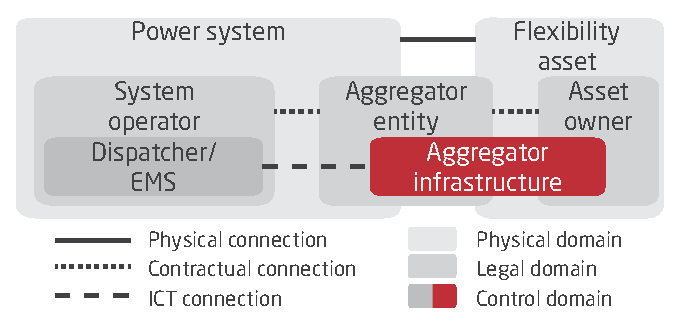
\includegraphics[width=1.0\textwidth]{etfa2015/domains.eps}
\caption{The aggregator concept across domains.}
\label{fig:MAINdomains}
%\vspace*{-5mm}
\end{figure}

These concepts lead to the following definitions:
\begin{description}
	\item[Aggregator role:] The role in the power system of performing aggregation with the purpose of selling the flexibility in consumption or production. The sale of flexibility can be a service to System Operators\footnote{The term System Operators is used here to refer to both Transmission System Operators and Distribution System Operators} or it can be traded in day ahead markets. Theaggregator role can be assigned to a new player in the markets, or it can be assigned to an existing player, e.g. a Balance Responsible Party or a utility.
	\item[Aggregator entity:] The legal entity of the aggregator, which enters into contractual agreements with the other market players and flexibility asset owners. This entity is legally responsible for living up to the contractual agreements.
	\item[Aggregator infrastructure:] The communication and control infrastructure, both in terms of software and hardware, that the aggregator owns and operates in order to control the flexibility assets.
	\item[Aggregator architecture:] The shape of the aggregator infrastructure. This encompasses not only the control strategy, but a series of essential functions which will be described in Section~\ref{sec:MAINaggrefarch}.
	\item[Aggregator:] The term used to refer to a market player that has an aggregator role, entity and infrastructure.
\end{description}

Aggregators provide two kinds of services\footnote{The terminology used in Appendices~\ref{app:etfa2015} and \ref{app:isgt2014} varies slightly from the one presented here. The terms used in this section are considered definitive.\bondy{I'm not sure the wording is right here}}:
\begin{description}
	\item[Flexibility services] which are provided to System Operators and BRPs. These will take the form of ancillary services for the TSO, distribution system services for the DSO and portfolio balancing services for the BRP\footnote{The mentioned types of services will be expanded upon in Chapter~\ref{cha:services}.}.
	\item[Asset management services] provided to the owners of the units.
\end{description}
This is shown in Figure~\ref{fig:market_futureMAIN}, where the aggregator is selling services to the System Operators through the Consumption BRP. This is a market setup which was concluded upon in the iPower project. Other market setups allow for the aggregator to participate directly in the market, as long as they coordinate with their corresponding Consumption BRP, such that the aggregator avoids provoking imbalances to the Consumption BRP.
\begin{figure}[htbp!]
\centering
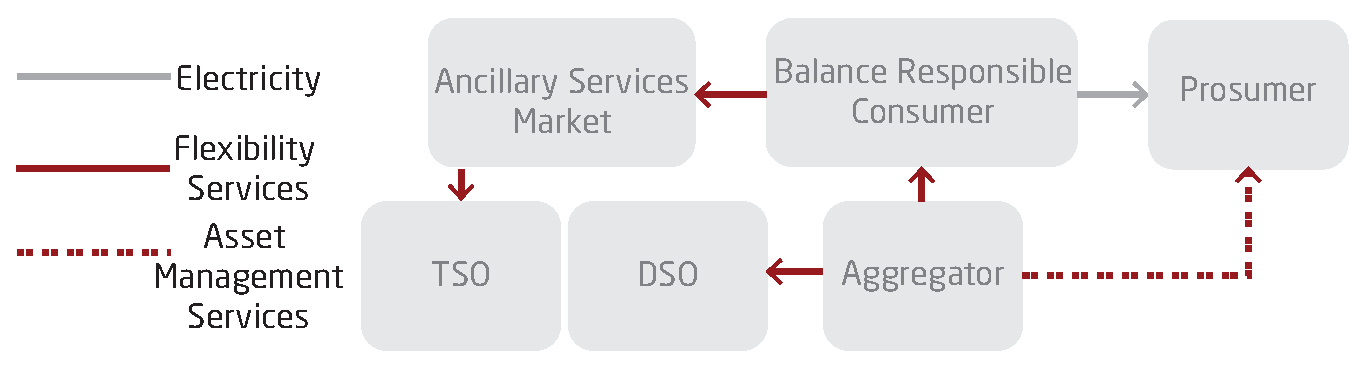
\includegraphics[width=1.0\textwidth]{market_futureMAIN.eps}
\caption{The aggregator as a service provider. This figure is a modified version of Figures~\ref{fig:marketfuture} and \ref{fig:SEGANmarket}.}
\label{fig:market_futureMAIN}
%\vspace*{-5mm}
\end{figure}

Another concept that needs to be defined is the one of \emph{flexibility}. The word has been used loosely as the amount of power consumption/production a unit is able to provide as a service. To expand upon this, two kinds of flexibility are considered: \emph{deferred} and \emph{non-deferred} flexibility. When flexibility is provided as a \emph{non-deferred} flexibility,  it means that the consumption/generation is reduced/increased without the need to recuperate/shed the energy provided in the service. Correspondingly, \emph{deferred} flexibility is where the units providing the service need to return to a nominal state by recuperating or shedding energy. In demand response, the latter is the most common kind of flexibility used. Consequently, flexibility has two dimensions:
\begin{itemize}
	\item a volume of power (or energy) that can be provided, and
	\item a time horizon over which the consumption/production can be changed.
\end{itemize} 

Finally, one of the central points of this work is that aggregators are essentially different from traditional generators. Aggregators differ from traditional generators in the sense that:
\begin{enumerate}
	\item they are distributed systems where each unit has its own response properties, therefore the overall response behaves very differently than that of traditional generators;\label{point:aggblackbox}
	\item they have no single point of measurement, which means the traditional measuring requirements can not be met;
	\item reliability concepts must be adapted to their distributed nature;
	\item aggregator architectures will vary widely, and each architecture will be sensitive to different operation scenarios.
\end{enumerate}

%While the dynamics of fossil-fueled power plants are well understood and can be modelled based upon physical equations, aggregators can only be analyzed as black boxes.
\section{Advantages and Limitations of Aggregators}
\newsection{A}{s stated in the} previous section, the aggregator is a cross-domain entity. Most of the literature on aggregators and demand response focuses on the advances in the control domain which bring \emph{operating}, \emph{planning} and \emph{economic} advantages to the power system\fcite{oconnell2014benefits}. In this work the focus is on the \emph{operating} advantages brought by aggregators, which can divided into three categories: \emph{scalability}, \emph{reliability} and \emph{responsiveness}.

In the control domain,\marginnote{The concepts described in this section are focused on aggregators as service providers, but the same concepts can be applied for aggregators trading in the day-ahead or intra-day markets} the advantages of contracting an aggregator instead of a large amount of individual small sized units are similar to those of the legal domain. That is, the aggregator in its essence can be regarded as a solution for \emph{scalability} of the smart control of flexible consumption or production. It would be possible for a System Operator to directly engage all customers in order to buy services, but the coordination of such large quantities is impractical for the System Operators. Thus, The System Operators can request fewer services with large volume, and the aggregator will then supply this service with its portfolio of units.

Aggregators providing services through demand response can be more reliable that their traditional counterpart\fcite{kirby2007a,callaway2011a}. This is due to the fact that a fault in one large generator will have a much higher impact than faults in several smaller-sized units. This makes for an argument for aggregators improving the \emph{reliability} of power system.\bondy{Should I reproduce the Kirby's figure here? Expand upon the idea?}

Lastly, most DERs have very fast response times, which means that compared to traditional coal-fueled power plants, aggregators are able to provide very fast services. This implies that frequency excursions can be stopped faster and at a higher frequency nadir\fcite{vrettos2015frequency}. This leads to system operators requiring smaller reserves for maintaining  the system security\fcite{makarov2008assessing}.

The main technical limitation on aggregators is that most DERs have as a main objective to satisfy the needs of it's owner, e.g. transportation in the case of EVs or heating in the case of HPs. Thus, the aggregator is constrained in its flexibility by the primary function of the DERs. Similarly, selling flexibility through aggregators is optional, so an aggregator must make a compelling business case for the DER owner to participate in the service markets.

Another technical limitation is directly related to the kind of flexibility the aggregator provides. In most cases the aggregator will use \emph{deferred} flexibility, where the units need to recuperate after the service delivery. If all units in the portfolio recuperate at the same time, the consumption spike that ensues may be a larger problem than the one the aggregator was contracted to solve. This is also known as the kick-back effect\bondy{ask Xue for references}. The problem of saturation can also be associated with this. DERs are usually only able to deliver services on short time horizons (compared to traditional generators) due to the limit size of the units. Once a minimum or maximum state has been reached, the flexibility of the unit disappears. This concept is represented can be represented as set of saturation curves\fcite{thavlov2015thesis}, where asking for large volumes of power means the units can only deliver for short time periods and vice versa.

A non-technical limitation comes from the market regulations. Market rules and ancillary service requirements are defined based on the capabilities of traditional generators. This means that aggregators are expected to behave as traditional generators, when they in essence are something completely different. This means that rules and requirements need to be changed if aggregators are to be fully exploited\footnote{This topic is addressed in depth in Chapter~\ref{cha:services}.}.

\section{The Functional Aggregator Reference Architecture}\label{sec:MAINaggrefarch}
\newsection{U}{ntil now, the discussion} on the aggregator has been focused on its role in the power system. In order to further the understanding of what an aggregator is, its functionality must be analyzed. One of the main contributions of the presented research is a \emph{Functional Reference Architecture for Aggregators}. The objective of creating a reference architecture is to address the issue of benchmarking and validation/certification of aggregators\footnote{This topic will be discussed in depth in Chapter~\ref{cha:validation}.}. The traditional approach to certification of generators can not be applied to aggregators, and therefore new methods must be designed. Part of this method is to verify that an aggregator possesses the essential functionality for effective service provision. This essential functionality is defined in the proposed reference architecture.

In order to formulate the aggregator reference architecture, a set of existing commercial and academic aggregators\footnote{The analyzed aggregators were: Open Energi\cite{openenergi}, PowerHub by DONG Energy\cite{powerhub}, Heterogenous Aggregator by Aalborg University\cite{rahnama2014evaluation} and the D-EMPC\cite{costanzo2013coordination}.}  were decomposed into their basic functionality. The resulting functions are\footnote{For detailed explanations of each function see Section~\ref{sec:funcdec}.}:

\begin{enumerate}[label=\Alph*]
	\item Service interface
	\item Performance Monitoring
	\item Supervision and Resource Handling
	\item Operator Interface
	\item Control
	\item Flexibility Monitoring
	\item Aggregator-internal Communication
	\item Client Management
	\item External Information services
	\item Asset Interface
	\item Knowledge Exchange
\end{enumerate}

These functions abstract from any kind of aggregator architecture implementation, and provide the building blocks for the functional reference architecture shown in Figure~\ref{fig:MAINrefarch}\footnote{The diagram is also presented in Appendix~\ref{app:etfa2015}.}. Arrows representing data flow were avoided in the design, since they presuppose a specific aggregator architecture. Given that the functional reference architecture must be as encompassing as possible, it should not reflect any specific aggregator architecture implementation, e.g. centralized or distributed aggregators. 
\begin{figure}[htb]
\centering
\includegraphics[width=1.0\textwidth]{"etfa2015/diag_simple"}
\caption{A visual representation of the proposed reference architecture. The symbols represent data types that are outputs to the functions.}
\label{fig:MAINrefarch}
\end{figure}

\section{Conclusions Regarding Aggregators}
\newsection{T}{he concept of aggregators} is widespread in the smart grid literature, but the interpretations of what an aggregator is varies widely. One of the contributions of this research that was presented in this chapter is to provide a common lexicon and reference architecture for aggregators so that discussion on the topic can be harmonized. This will hopefully lead to faster advances in the field. Also, the functional reference architecture is to be used in aggregator validation and certification. A secondary use for the reference architecture is to serve as a guide for future designs of aggregators.

A current shortcoming of this work is that the presented functional reference architecture for aggregators is part of a work-in-progress paper and as such, needs to be refined and extended. Future work will include the design of key performance indices (KPIs) assigned to each function, such that the scores can be used for benchmarking. 

The next chapter will present a deeper analysis and justification for aggregator validation and certification.
% chapter The Aggregator (end)
